% CHAPITRE 4
\chapter{Effets de l'hydrologie sur les flux de CO2 et CH4}

\minitoc

\newpage

\section{Manipulation du niveau de l'eau en mésocosmes}
\section{Introduction}
\subsection{Procédure expérimentale}

\begin{figure}
\centering
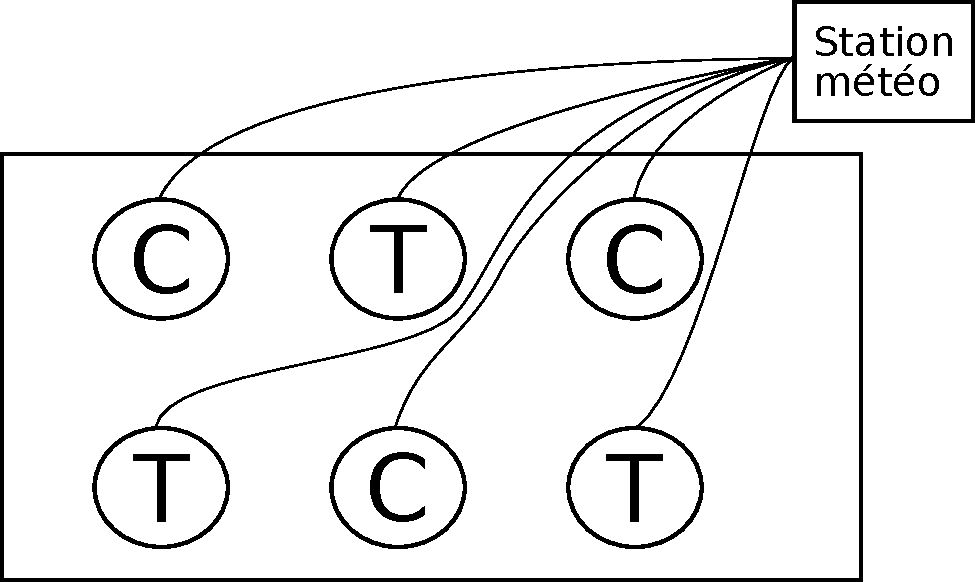
\includegraphics[width=.5\textwidth]{chap4/mesocarte}
\caption{Carte mésocosmes Zi}
\label{fig:mesocarte}
\end{figure}

\begin{figure}
\centering
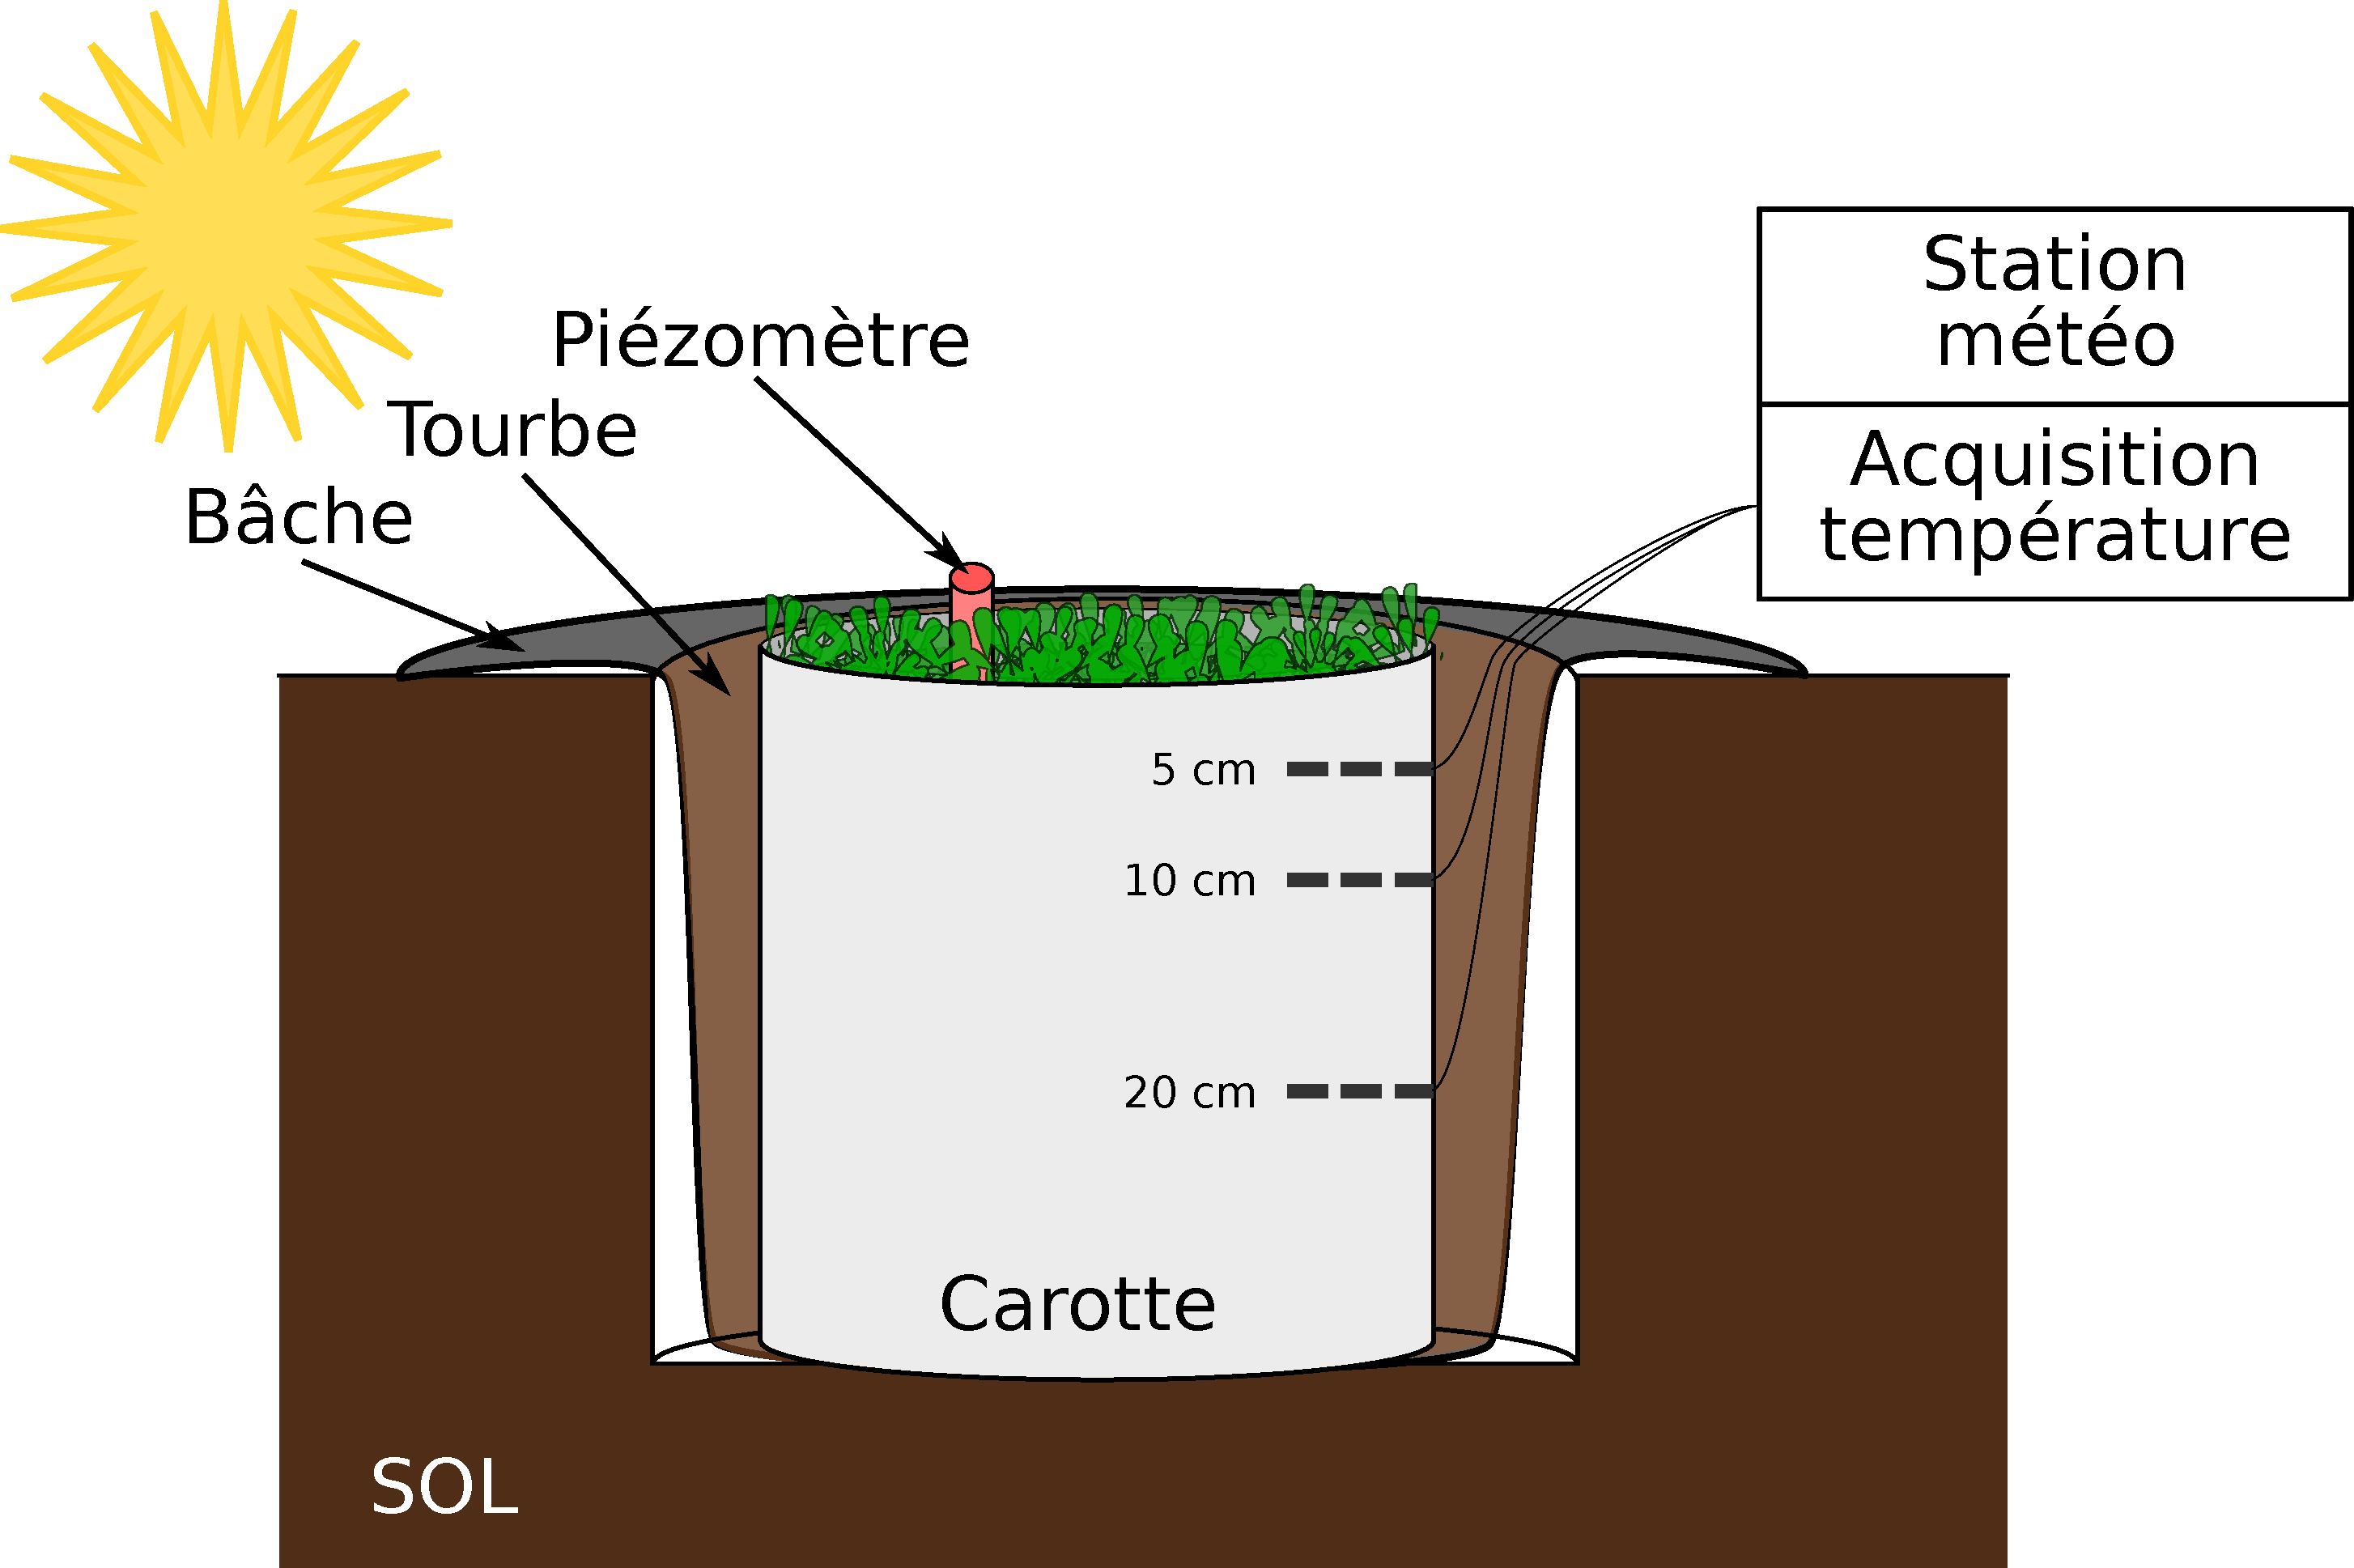
\includegraphics[width=.5\textwidth]{chap4/mesoinstall}
\caption{Schéma d'un mésocosme}
\label{fig:mesoinstall}
\end{figure}

\subsection{Résultats}

\begin{figure}
\centering
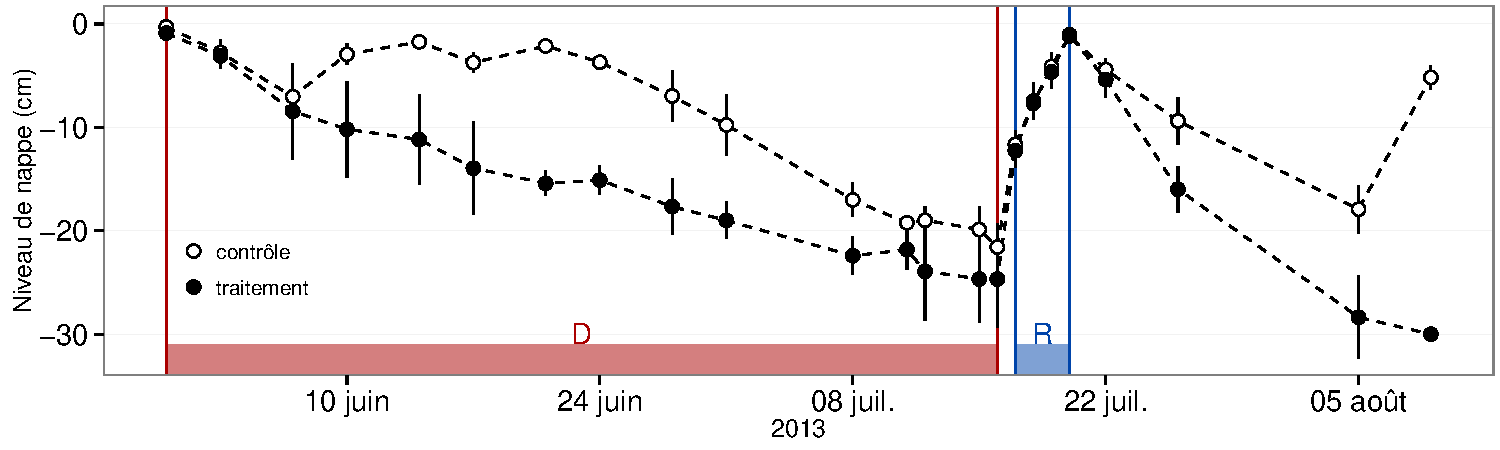
\includegraphics[width=\textwidth]{chap4/HMzi_wtl}
\caption{Évolution du niveau de la nappe dans les mésocosmes Zi}
\label{fig:HMzi_wtl}
\end{figure}

\begin{figure}
\centering
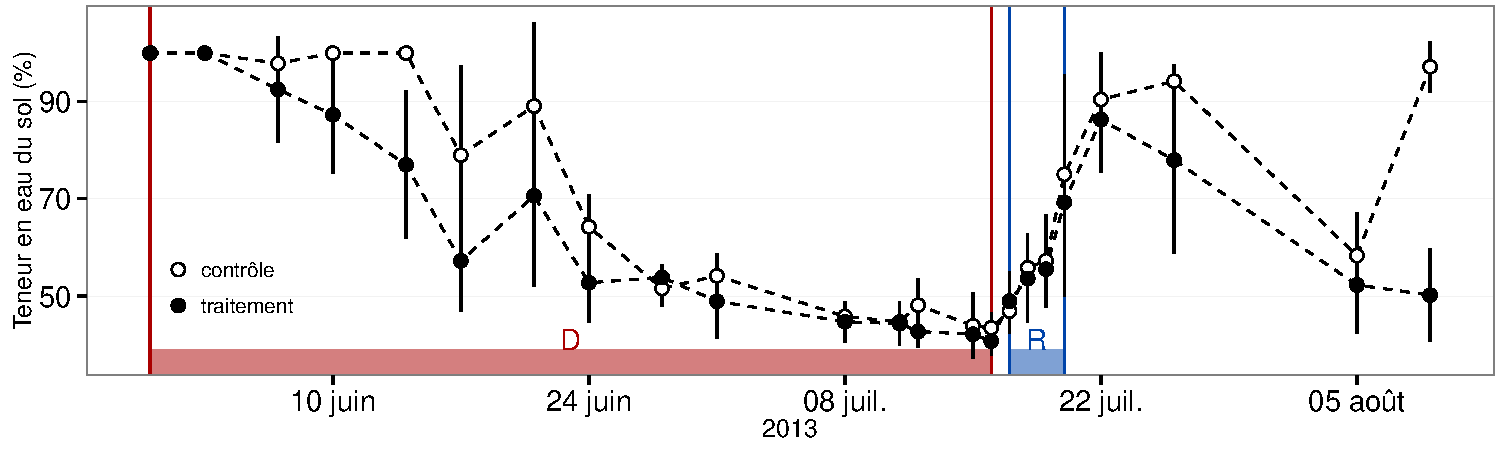
\includegraphics[width=\textwidth]{chap4/HMzi_TES}
\caption{Évolution de la teneur en eau du sol dans les mésocosmes Zi}
\label{fig:HMzi_TES}
\end{figure}

\begin{figure}
\centering
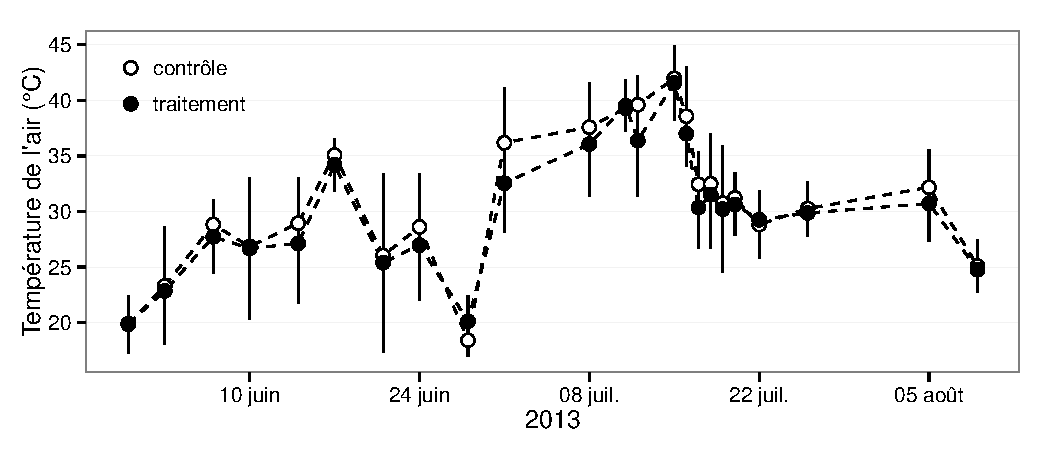
\includegraphics[width=\textwidth]{chap4/HMzi_Tair}
\caption{Évolution de la température de l'air dans les mésocosmes Zi}
\label{fig:HMzi_Tair}
\end{figure}

\begin{figure}
\centering
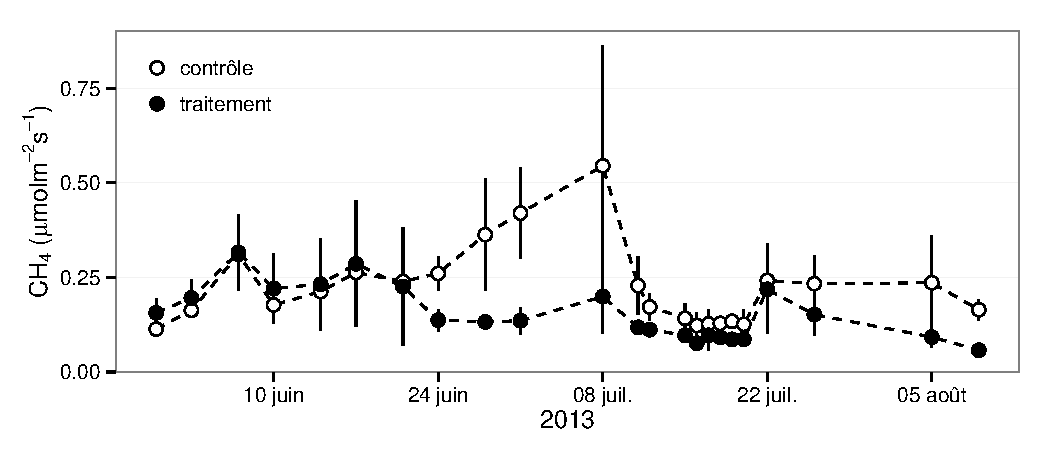
\includegraphics[width=\textwidth]{chap4/HMzi_ch4}
\caption{Évolution du méthane dans les mésocosmes Zi}
\label{fig:HMzi_ch4}
\end{figure}

\begin{figure}
\centering
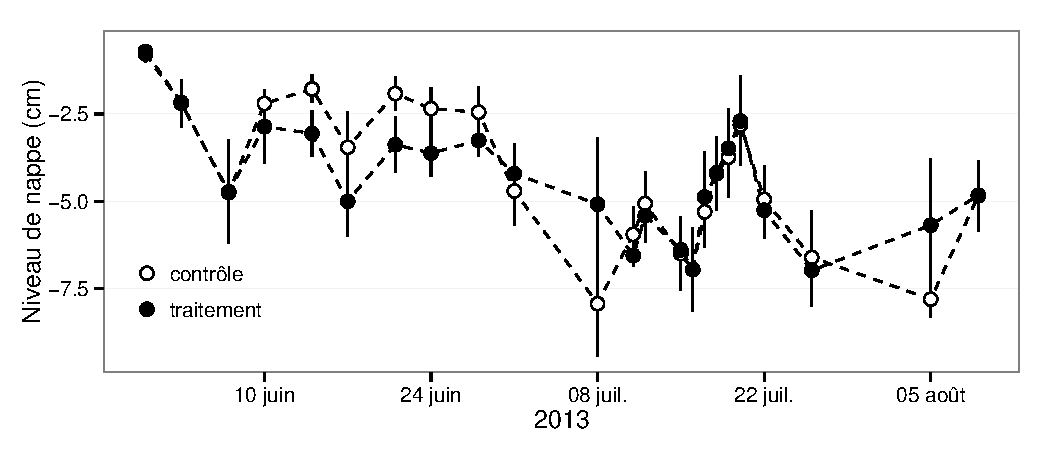
\includegraphics[width=\textwidth]{chap4/HMzi_ER}
\caption{Évolution de la RE dans les mésocosmes Zi}
\label{fig:HMzi_ER}
\end{figure}

\begin{figure}
\centering
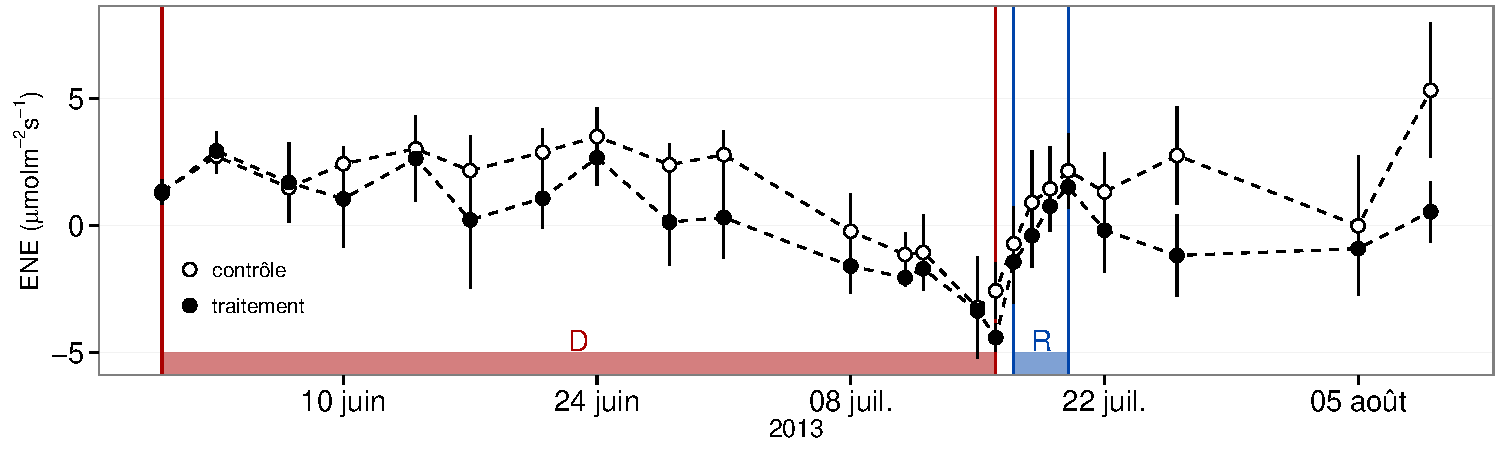
\includegraphics[width=\textwidth]{chap4/HMzi_NEE}
\caption{Évolution de la NEE dans les mésocosmes Zi}
\label{fig:HMzi_NEE}
\end{figure}


\begin{figure}
\centering
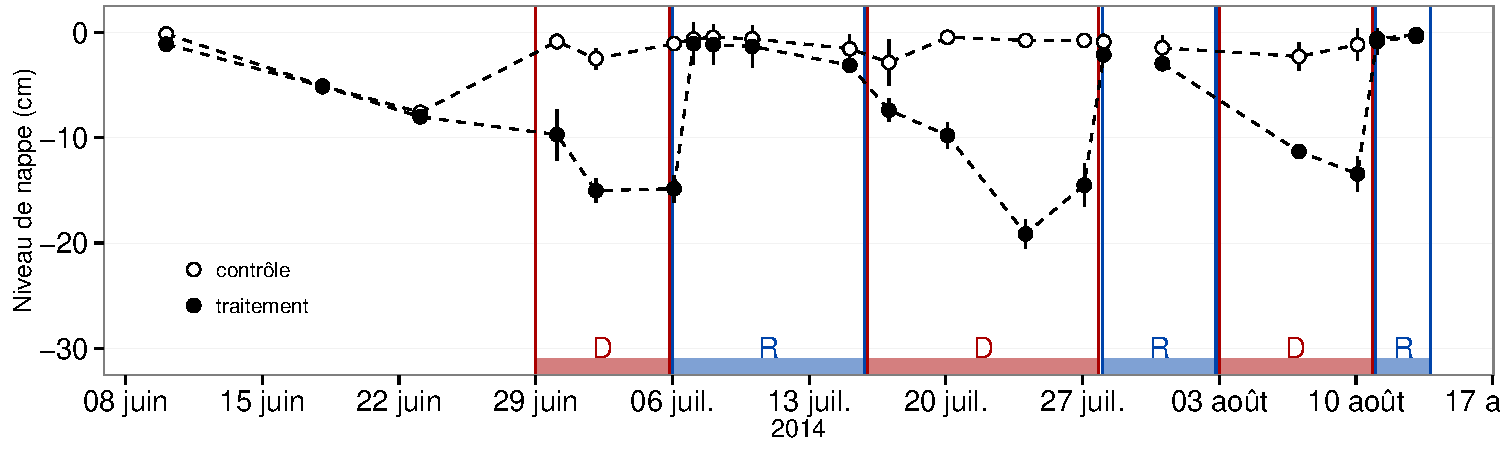
\includegraphics[width=\textwidth]{chap4/HMty_wtl}
\caption{Évolution du niveau de la nappe dans les mésocosmes Tianyi}
\label{fig:HMty_wtl}
\end{figure}

\begin{figure}
\centering
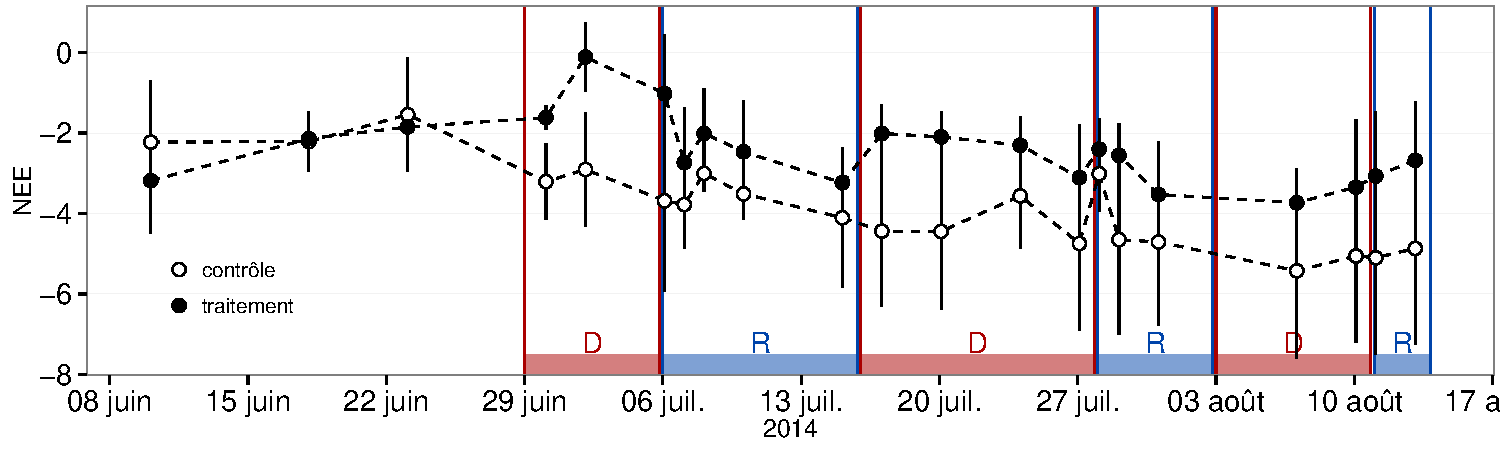
\includegraphics[width=\textwidth]{chap4/HMty_NEE}
\caption{Évolution de la NEE dans les mésocosmes Tianyi}
\label{fig:HMty_NEE}
\end{figure}

\begin{figure}
\centering
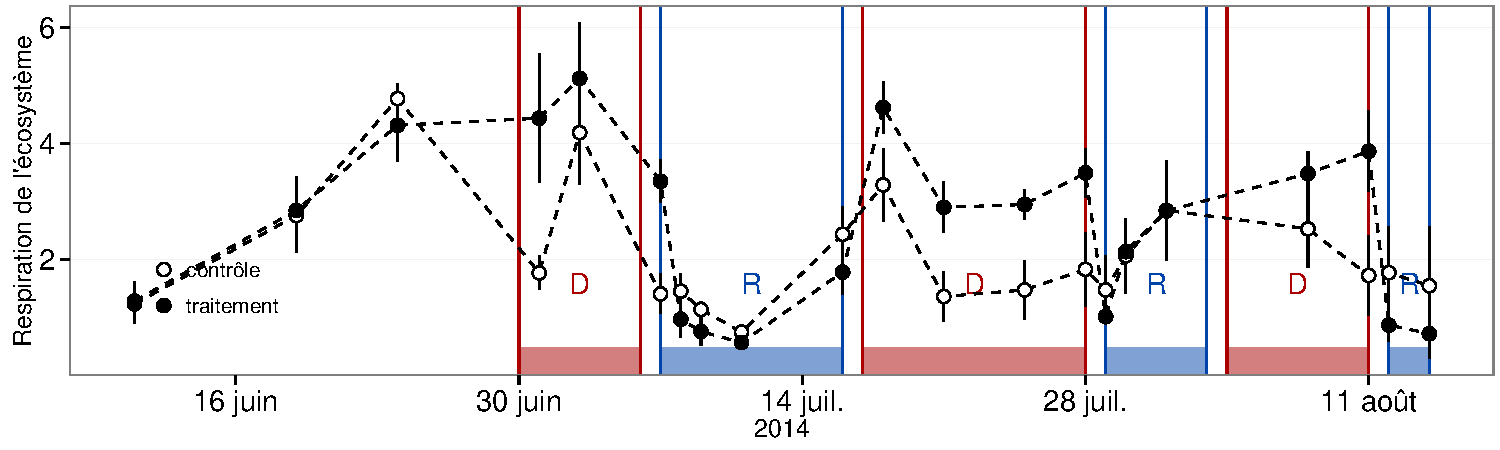
\includegraphics[width=\textwidth]{chap4/HMty_ER}
\caption{Évolution de la RE dans les mésocosmes Tianyi}
\label{fig:HMty_ER}
\end{figure}

\subsubsection{Dessication}

\begin{itemize}
\item augmentation RE
\item diminution CH4
\end{itemize}

\subsubsection{Événement pluvieux}

\begin{itemize}
\item diminution RE
\item augmentation CH4 avec retard
\end{itemize}

\subsubsection{Effet cycles multiples}

\subsection{Discussion}

%\section{Manipulation du niveau de l'eau (teneur en eau) in-situ}
%\subsection{introduction}
%L'étude des effets de l'hydrologie sur les émissions de flux de GES a également pu être menée directement in-situ au sein du projet CARBIODIV (Restauration hydrologique de la tourbière de La Guette : effets sur l'évolution de la biodiversité et le stockage du carbone.) dont l'objectif est de restaurer le fonctionnement hydrologique de la tourbière de La Guette.
%\subsection{Procédure expérimentale}
%\subsubsection{Les travaux}
%\subsubsection{Les stations scientifiques}
%Deux stations ont été installées sur le site, dans deux sous-hydrosystèmes différents. Le premier en amont n'étant pas impacté par les travaux permet de contrôler les effets de site, et le second, en aval, enregistrera les effets de la restauration hydrologique.
%\subsection{Résultats}
%\subsection{Discussion}
